\documentclass{article}%
\usepackage[T1]{fontenc}%
\usepackage[utf8]{inputenc}%
\usepackage{lmodern}%
\usepackage{textcomp}%
\usepackage{lastpage}%
\usepackage[head=40pt,margin=0.5in,bottom=0.6in]{geometry}%
\usepackage{graphicx}%
%
\title{\textbf{Estas son las fotos sobre Venezuela que colocaron en el Senado de EE UU}}%
\author{El Nacional}%
\date{07/03/2019}%
%
\begin{document}%
\normalsize%
\maketitle%
\textbf{URL: }%
http://www.el{-}nacional.com/noticias/estas{-}son{-}las{-}fotos{-}sobre{-}venezuela{-}que{-}colocaron{-}senado\_273732\newline%
%
\textbf{Periodico: }%
EN, %
ID: %
273732, %
Seccion: %
EE UU\newline%
%
\textbf{Palabras Claves: }%
Política, Estados Unidos, Crisis humanitaria\newline%
%
\textbf{Derecho: }%
2.1%
, Otros Derechos: %
\newline%
%
\textbf{\textit{Este jueves se realiza una audiencia sobre la relación de Estados Unidos y Venezuela}}%
\newline%
\newline%
%
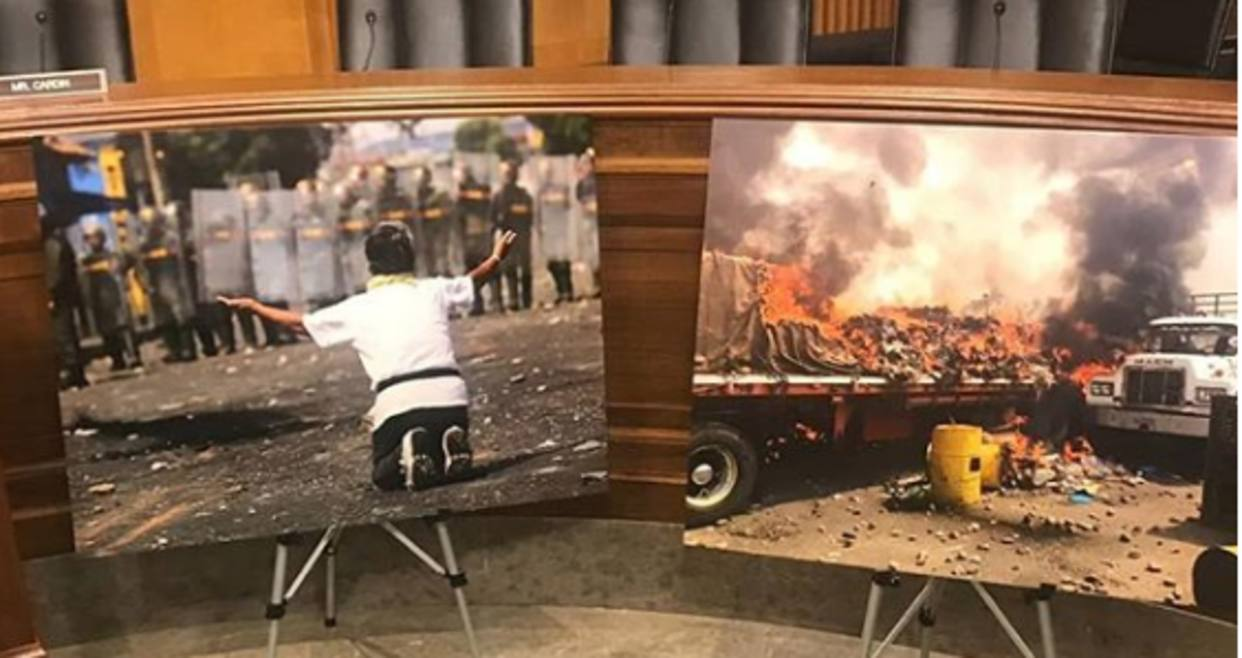
\includegraphics[width=300px]{EN_273732.jpg}%
\newline%
%
En la sede del Senado de los Estados Unidos colocaron diversas fotos sobre momentos recientes políticos y sociales de Venezuela~en~los últimos meses.%
\newline%
%
En una de las fotos se observa el camión en el que se quemó la ayuda humanitaria y otra de las imágenes~retrata el momento de uno de los ataques de represión. En una de las gráficas también aparece el presidente interino, Juan Guaidó, levantando el pulgar en una de las movilizaciones.%
\newline%
%
Este jueves se realiza en el Senado una audiencia sobre las relaciones de EE UU con Venezuela, en la que participan diversos venezolanos que llegaron proveniente de 23 estados de la nación norteamericana.%
\newline%
%
\end{document}